\documentclass[a4paper]{article}
\usepackage[pagebackref=false,colorlinks,linkcolor=black,citecolor=magenta]{hyperref}

\usepackage{indentfirst}
\usepackage{geometry}
\usepackage{enumitem}
\usepackage{amsmath}
\usepackage[usenames,dvipsnames]{color,xcolor}
\definecolor{mygreen}{RGB}{28,172,0} % color values Red, Green, Blue
\definecolor{mylilas}{RGB}{170,55,241}
\usepackage{listings}
\usepackage{hyperref}
\hypersetup{linkcolor=red}
\usepackage{graphicx}
\usepackage{emptypage}
\usepackage{afterpage}
\usepackage{titlesec}

\titleformat{\section}
{\normalfont\fontsize{20}{20}\bfseries}{\thesection}{1em}{}

\titleformat{\subsection}
{\normalfont\fontsize{15}{20}\bfseries}{\thesubsection}{1em}{}

\titleformat{\subsubsection}
{\normalfont\fontsize{12}{20}\bfseries}{\thesubsubsection}{1em}{}

\usepackage{pdfpages}
\usepackage{tikz}
\usepackage[american]{circuitikz}
\renewcommand{\baselinestretch}{1.2} 
\lstset{language=Python,%
	%basicstyle=\color{red},
	breaklines=true,%
	morekeywords={matlab2tikz},
	keywordstyle=\color{blue},%
	morekeywords=[2]{1}, keywordstyle=[2]{\color{black}},
	identifierstyle=\color{black},%
	stringstyle=\color{mylilas},
	commentstyle=\color{mygreen},%
	showstringspaces=false,%without this there will be a symbol in the places where there is a space
	numbers=left,%
	numberstyle={\tiny \color{black}},% size of the numbers
	numbersep=9pt, % this defines how far the numbers are from the text
	emph=[1]{for,end,break},emphstyle=[1]\color{blue}, %some words to emphasise
	%emph=[2]{word1,word2}, emphstyle=[2]{style},    
}

\geometry{
	a4paper,
	total={170mm,257mm},
	left=20mm,
	top=20mm,
}
\usepackage{fancyhdr}
\pagestyle{fancy}
\fancyhf{}
\rhead{\textbf{درس علوم اعصاب: یادگیری، حافظه، شناخت}}
\lhead{\textbf{پروژه اول-آموزش شبکه‌های عصبی بازگشتی انگیزشی-بازدارنده}}
\cfoot{(\space \space \space \space \textbf{\thepage}  \space \space \space)}
\renewcommand{\headrulewidth}{1pt}
\renewcommand{\footrulewidth}{1pt}
\setlength{\parindent}{0ex}
\setlength{\parskip}{0ex}


\usepackage{xepersian}
%\setlatintextfont[Scale=1]{Times New Roman}
\settextfont{XB Niloofar}
\setdigitfont{XB Niloofar}
\DefaultMathsDigits 

\begin{document}
	
\begin{titlepage}
	
	\begin{center}
		\textbf{
			باسمه تعالی\\
		}
		\vspace{1cm}
		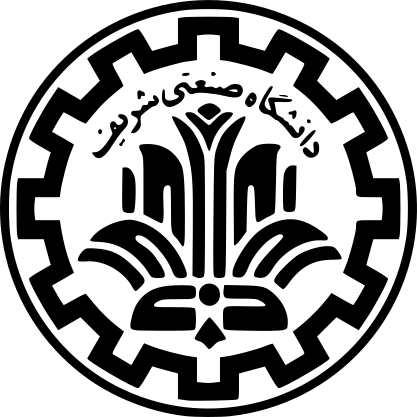
\includegraphics[scale=0.25]{logo.png}\\
		\vspace{0.5cm}
		\begin{Large}
			\textbf{
				دانشگاه صنعتی شریف\\
				\vspace{0.5cm}
				دانشکده مهندسی برق\\
			}
		\end{Large}
		\vspace{1.5cm}
		\begin{huge}
			\textbf{
				درس علوم اعصاب: یادگیری، حافظه، شناخت\\
				\vspace{0.5cm}
				پروژه اول\\
				\vspace{0.5cm}
				آموزش شبکه‌های عصبی بازگشتی انگیزشی-بازدارنده\\
				\LARGE
		\lr{(Excitatory-Inhibitory Recurrent Neural Networks)}\\
	}
		\end{huge}
		\vspace{1.5cm}
		\begin{Large}
			\textbf{
				استاد درس: دکتر کربلایی آقاجان\\
				\vspace{1.5cm}
				امیرحسین افشارراد\\
				\vspace{0.5cm}
				۹۵۱۰۱۰۷۷\\
				\vspace{1cm}
				محمدمهدی ابوالحسنی\\
				\vspace{0.5cm}
				95100983\\
				\vspace{2cm}
				\today
			}
		\end{Large}
		
	\end{center}
	
	\thispagestyle{empty}
\end{titlepage}	

	\large
\section{مقدمه و معرفی مدل}
\subsection{تصحیح مدل مورد استفاده در تمرین قبل}
ابتدا برای شروع به انجام شبیه‌سازی‌های مربوط به این پروژه، اقدام به تصحیح و تکمیل مدل مورد استفاده در تمرین قبل کردیم. در نتیجه‌ی این اقدام، خروجی‌های مطلوب حاصل شدند و دو مشکل اصلی مرتفع شد؛ اول مشکل عدم ارائه‌ی پاسخ صحیح توسط شبکه در تشخیص بیت پریتی که ناشی از عدم انجام کامل فرایند 
\lr{backpropagation}
بود؛ و دیگر مشکل بریده شدن خروجی سیگنال‌های سینوسی در مقادیر $1$ و $-1$ که ناشی از وجود تابع فعال‌سازی 
\lr{tanh}
بود.
قطعه کد زیر مدل این شبکه را نشان می‌دهد:
 \begin{normalsize}
	\begin{latin}
		\texttt{\lstinputlisting{code01.py}}
	\end{latin}
\end{normalsize}

\subsection{تکمیل مدل بر مبنای مقاله‌ی مرجع}
مدل مذکور در قسمت قبل با انجام تغییرات اندکی، به مدل جدید و مطلوب تبدیل می‌شود. معادله \ref{eq01} رابطه‌ای است که مبنای تعریف مدل مورد استفاده در این پروژه است.

	\begin{equation}
{\mathbf{x}_t} = (1-\alpha)\mathbf{x_{t-1}}+\alpha(W^{rec}\mathbf{r_{t-1}}+W^{in}\mathbf{u_t})+\sqrt{2\alpha\sigma^2_{rec}}\boldsymbol{N}(0,1) 
\label{eq01}
\end{equation}

در اثر اعمال تغییرات، کد مورد استفاده برای تعریف مدل به شکل زیر در می‌آید:
 \begin{normalsize}
	\begin{latin}
		\texttt{\lstinputlisting{code02.py}}
	\end{latin}
\end{normalsize}

نکته‌ی قابل ذکر این است که به منظور پیاده‌سازی تسک‌هایی که خروجی‌های آن‌ها مقادیر باینری هستند، یک تابع غیرخطی 
\lr{tanh}
 نیز به مدل اضافه شده است. ضمناً شایان ذکر است، به منظور ساده‌تر شدن مدل (و با پرسش از دستیار آموزشی درس) از نویز موجود در داخل نورون‌ها صرف نظر کردیم و صرفاً از ورودی‌های دارای نویز استفاده کردیم.\\
 مورد دیگری که نیاز به انجام داشت تا به مدل توصیف‌شده در مقاله دست یابیم، تشکیل دسته‌های جداگانه‌ی نورون‌های انگیزشی و بازدارنده بود. این کار متناظر با آن است که بخشی از ستون‌های ماتریس وزن شبکه، مقادیر تماماً مثبت (یا صفر) و بخش دیگر، مقادیر تماماً منفی (یا صفر) داشته باشد. همچنین قطر اصلی ماتریس وزن نیز باید صفر باشد. می‌توان این محدودیت‌ها را در تعریف اولیه‌ی مدل اعمال کرد، اما روشی که ما در این پروژه مورد استفاده قرار دادیم، به شرح زیر است:\\
 در فرایند آموزش شبکه، هر بار که وزن‌های شبکه بروزرسانی می‌شوند، محدودیت‌های مطلوب را روی آن‌ها اعمال می‌کنیم. به عبارت دقیق‌تر، پس از هر بروزرسانی وزن‌ها، قطر اصلی ماتریس وزن را صفر کرده و مقادیر $80\%$ از این ماتریس را با اعمال قدر مطلق مثبت کرده، و مقادیر باقیمانده را با روش مشابه به اجبار به مقادیر منفی (یا صفر) تبدیل می‌کنیم. قطعه کدی که این کار را انجام می‌دهد در ادامه قابل مشاهده است:
 \begin{normalsize}
 	 \begin{latin}
 		\texttt{\lstinputlisting{code03.py}}
 	\end{latin}
 \end{normalsize}
 همچنین یک نمونه از ماتریس‌های وزن پس از اعمال تغییرات مذکور در شکل \ref{fig02} قابل مشاهده است. (با کمی دقت) می‌توان مشاهده کرد که قطر اصلی تماماً صفر است و دو ستون انتهایی، مقادیری کمتر یا مساوی صفر دارند، در حالی که هشت ستون اول دارای مقادیر نامنفی‌اند.
 \begin{figure}[h!]
 	\centering
 	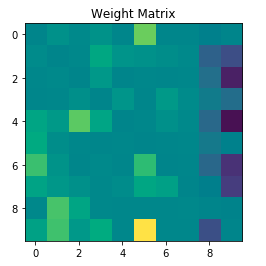
\includegraphics[scale=0.7]{fig02.png}
 	\caption{ماتریس وزن با محدودیت‌ صفر بودن قطر اصلی و وجود نورون‌های انگیزشی و بازدارنده}
 	\label{fig02}
 \end{figure}
 
 \section{تسک اول: 
 \lr{Perceptual Decision Making}}
این تسک در متن مقاله به دو شکل متفاوت پیاده‌سازی شده است که در این جا به بررسی هر دو روش می‌پردازیم. در ادامه نیز اتصالات شبکه را به گونه‌ای (که در ادامه توضیح داده خواهد شد) تغییر می‌دهیم و با یک روش سوم نیز به پیاده‌سازی مسأله می‌پردازیم.

\subsection{تولید دیتاست}
آزمایش مرجع مربوط به این بخش، آزمایش حرکت تصادفی نقاط بوده است. برای مدل‌سازی این آزمایش، نیاز داریم درصد حرکت نقاط در دو جهت مختلف را به گونه‌ای در ورودی مدل کنیم. می‌دانیم که در آزمایش اصلی، هرچقدر درصد نقاطی که در یک جهت حرکت می‌کنند بیشتر باشد، استنتاج برای تعیین جهت حرکت عمومی نقاط ساده تر است. برای مدل کردن این رفتار، از دو مقدار ثابت استفاده می‌کنیم که نماد درصد حرکت نقاط هستند؛ بنابراین هر چه این دو مقدار به یک‌دیگر نزدیک‌تر باشند، تصمیم‌گیری سخت‌تر خواهد بود. به منظور پیاده‌سازی این دیتاست، تابع \texttt{decision\_making\_dataset} نوشته شده و در کد مرجع موجود است.\\
یک نکته‌ی مهم آن است که در متن مقاله زمان شروع ورودی به شبکه اعلام می‌شود که ما برای سادگی، تحریک را از لحظه‌ی صفر می‌دهیم و این ورودی را حذف می‌کنیم.
\subsection{پیاده‌سازی اول: تصمیم‌گیری پس از مشاهده کل ورودی}
در این پیاده‌سازی،‌ شبکه پس از مشاهده‌ی تمام ورودی‌ها، تصمیم خود را برای انتخاب یکی از دو ورودی (متناظر با یکی از دو جهت در آزمایش اصلی) اعلام می‌کند. طبق تعریف اولیه‌ی شبکه، پس از اعمال هر ورودی در واحد زمان، شبکه یک خروجی اعلام می‌کند. برای سهولت و یک‌پارچگی بیشتر، تعریف اولیه شبکه را تغییر نمی‌دهیم و به همین شکل باقی می‌گذاریم؛ و نحوه‌ی استفاده‌ی خود از شبکه را به گونه‌ی مطلوب تنظیم می‌کنیم. برای این کار، پس از اتمام هر ورودی در طول زمان، تنها آخرین خروجی را مد نظر قرار می‌دهیم و با مقایسه‌ی آن با خروجی مطلوب، وزن‌ها را بروزرسانی می‌کنیم. دقت کنید که خروجی‌ها دو بیتی هستند که یکی صفر و دیگری یک است که نشان‌دهنده‌ی تصمیم شبکه است. شکل \ref{fig01} نمودار درصد پاسخ‌گویی شبکه روی داده‌ی تست را به ازای تحریک‌هایی با طول مختلف (نمودارهای مختلف) و به ازای مقادیر مختلف تفاوت دو ورودی (هر نمودار) نشان می‌دهد. مشاهده می‌شود که با افزایش تفاوت دو مقدار، درصد پاسخ‌گویی زیاد می‌شود. همچنین به طور تقریبی مشاهده می‌شود که افزایش طول تحریک نیز موجب بهبود نتایج می‌گردد.
\begin{figure}[h!]
	\centering
	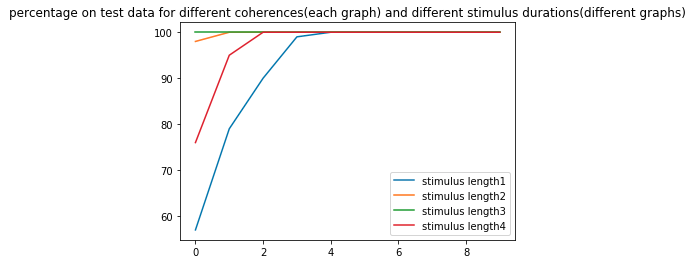
\includegraphics[scale=0.7]{fig01.png}
	\caption{نمودارهای درصد پاسخ صحیح دیتای تست برای طول‌های مختلف تحریک و تفاوت مقادیر دو تحریک}
	\label{fig01}
\end{figure}

\subsection{پیاده‌سازی دوم: تصمیم‌گیری به محض رسیدن به تصمیم قطعی}
در دومین پیاده‌سازی مربوط به این بخش، شبکه نیازی به صبر کردن تا انتهای ورودی را ندارد و به محض این که به تصمیم قطعی برسد، تصمیم خود را اعمال می‌کند. برای پیاده‌سازی این فرایند، شرط تصمیم قطعی را به این شکل تعریف کردیم: اگر خروجی شبکه در سه واحد زمانی متوالی یکسان باشد، شبکه به تصمیم قطعی رسیده است.\\
واضح است که می‌توان تعاریف دیگری را نیز برای این مدل‌سازی در نظر گرفت.\\
شکل‌های \ref{fig03} و \ref{fig04} به ترتیب زمان واکنش شبکه به ازای مقادیر مختلف تفاوت مقدار تحریک‌ها، و نیز درصد پاسخ صحیح شبکه در این شرایط را نمایش می‌دهند. مشاهده می‌شود که با افزایش تفاوت دو ورودی، سرعت پاسخ شبکه و نیز دقت آن افزایش می‌یابد.

\begin{figure}[h!]
	\centering
	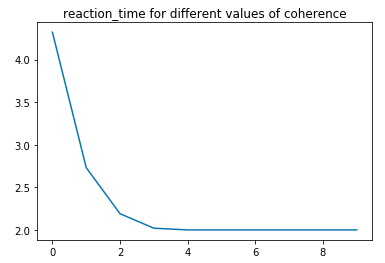
\includegraphics[scale=0.7]{fig03.png}
	\caption{زمان واکنش شبکه به ازای مقادیر مختلف تفاوت مقدار دو تحریک}
	\label{fig03}
\end{figure}


\begin{figure}[h!]
	\centering
	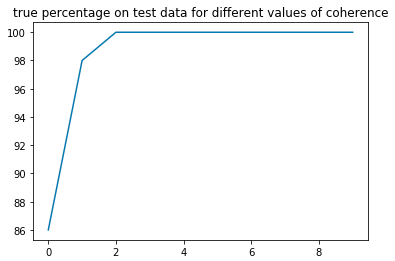
\includegraphics[scale=0.7]{fig04.png}
	\caption{درصد پاسخ صحیح شبکه به دیتای تست برای مقادیر مختلف تفاوت مقدار دو تحریک}
	\label{fig04}
\end{figure}

\subsection{پیاده‌سازی دوم: محدودیت الگوی اتصال نورون‌ها}
در این بخش، اتصالات نورون‌ها را محدود می‌کنیم، به گونه‌ای که نورون‌های دریافت‌کننده‌ی ورودی اول و دوم جدا باشند. بنابراین بین این نورون‌ها اتصالی وجود نخواهد داشت تصمیم‌گیرندگان مربوط به هر یک از دو ورودی جدا خواهند بود. در این حالت شکل‌های \ref{fig06}، \ref{fig05}، و \ref{fig07} به ترتیب نشان‌گر ماتریس اتصالات ورودی به لایه‌ی درونی، ماتریس اتصالات درونی، و ماتریس اتصالات لایه‌ی درونی به خروجی می‌باشند. مشاهده می‌شود که در این حالت مقادیر صفر در نواحی معینی از این ماتریس‌ها وجود دارد. برای مشخص شدن بهتر موضوع، شکل \ref{fig08} را در نظر بگیرید که شکل متناظر با این فرایند در مقاله‌ی مرجع است.
\begin{figure}[h!]
	\centering
	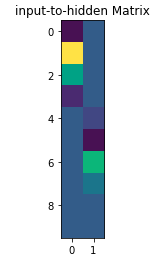
\includegraphics[scale=0.7]{fig06.png}
	\caption{ماتریس اتصالات ورودی به لایه‌ی درونی}
	\label{fig06}
\end{figure}

\begin{figure}[h!]
	\centering
	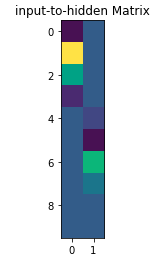
\includegraphics[scale=0.7]{fig06.png}
	\caption{ماتریس اتصالات درونی}
	\label{fig05}
\end{figure}

\begin{figure}[h!]
	\centering
	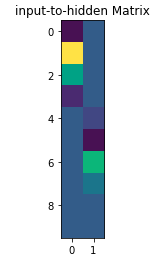
\includegraphics[scale=0.7]{fig06.png}
	\caption{ماتریس اتصالات لایه‌ی درونی به خروجی}
	\label{fig07}
\end{figure}

\begin{figure}[h!]
	\centering
	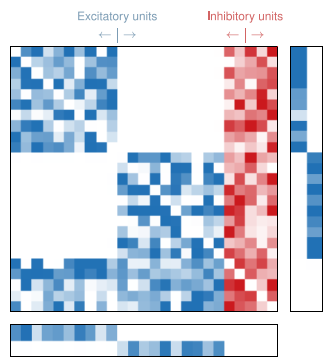
\includegraphics[scale=0.7]{fig08.png}
	\caption{شکل موجود در مقاله‌ی مرجع متناظر با شکل‌های \ref{fig06} و \ref{fig05} و \ref{fig07}}
	\label{fig08}
\end{figure}
	در این حالت میزان زمان واکنش و درصد پاسخ صحیح آن برای مقادیر مختلف تفاوت مقدار دو ورودی در شکل‌های \ref{fig09} و \ref{fig10} قابل مشاهده است. مجدداً مشاهده می‌شود که افزایش تفاوت دو ورودی موجب افزایش سرعت و دقت شبکه در پاسخ‌گویی می‌شود.
\begin{figure}[h!]
	\centering
	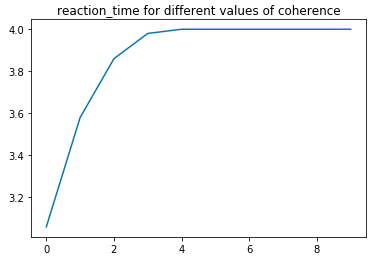
\includegraphics[scale=0.7]{fig09.png}
	\caption{زمان واکنش شبکه به ازای مقادیر مختلف تفاوت مقدار دو تحریک}
	\label{fig09}
\end{figure}

\begin{figure}[h!]
	\centering
	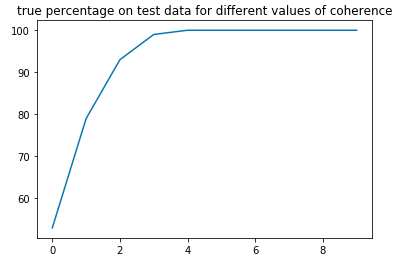
\includegraphics[scale=0.7]{fig10.png}
	\caption{درصد پاسخ صحیح شبکه به دیتای تست برای مقادیر مختلف تفاوت مقدار دو تحریک}
	\label{fig10}
\end{figure}

\section{تسک دوم: \lr{Parametric Working Memory }}
این تسک مربوط به مقایسه‌ی دو فرکانس مختلف و انتخاب فرکانس بالاتر است. تفاوت این تسک با تسک قبلی در آن است که این بار، دو ورودی نه به صورت هم‌زمان، بلکه به صورت متوالی (و با وجود یک وقفه‌ی کوتاه بین دو ورودی) به شبکه اعمال می‌شوند. 
\subsection{تولید دیتاست}
برای مدل کردن این ورودی‌ها، طبق توضیح مقاله، از دو مقدار عددی (همراه با نویز) استفاده می‌کنیم. نمونه‌ای از ورودی‌های تولیدشده در شکل \ref{fig11} قابل مشاهده است.
\begin{figure}[h!]
	\centering
	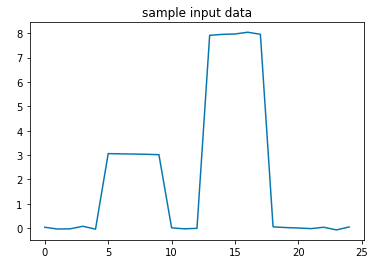
\includegraphics[scale=0.7]{fig11.png}
	\caption{نمونه‌ای از ورودی‌های اعمال‌شده به شبکه در تسک حافظه‌ی کاری}
	\label{fig11}
\end{figure}

\subsection{پیاده‌سازی تسک}
پیاده‌سازی این تسک به صورت اعمال یک ورودی (شکل \ref{fig11}) به شبکه و دریافت دو خروجی است که متناظر با مقدار (فرکانس) اول و مقدار (فرکانس) دوم هستند؛ بنابراین هر کدام از این دو که توسط شبکه بزرگ‌تر شناخته شوند، در خروجی مقدار یک خواهند داشت و دیگری دارای مقدار صفر خواهد بود. شکل \ref{fig12} درصد پاسخ صحیح شبکه را به دیتای تست برای مقادیر مختلف تفاوت مقدار دو تحریک نشان می‌دهد. مشاهده می‌شود که با افزایش تفاوت مقدار دو تحریک (تفاوت در فرکانس)، تصمیم‌گیری برای شبکه راحت‌تر شده و درصد پاسخ صحیح بیش‌تر می‌شود.
\begin{figure}[h!]
	\centering
	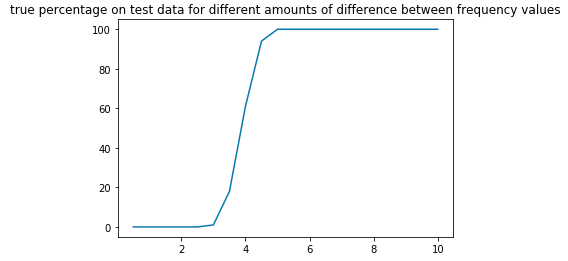
\includegraphics[scale=0.7]{fig12.png}
	\caption{درصد پاسخ صحیح شبکه به دیتای تست برای مقادیر مختلف تفاوت مقدار دو تحریک}
	\label{fig12}
\end{figure}

\section{تسک سوم: \lr{Eye-Movement Sequence Execution }}
در این تسک، مدل دنبال کردن حرکت یک نقطه توسط چشم را پیاده‌سازی می‌کنیم. خروجی شبکه باید محل چشم باشد که با دو مختص $x$ و $y$ مدل می‌شود.

\subsection{تولید دیتاست}
توضیحات مربوط به چگونگی تولید دیتاست در مقاله به صورت دقیق داده شده است. دیتاست شامل دو بخش است، یک بخش ۹ ورودی که متناظر با ۹ محل موجود در صفحه است؛ و بخش دیگر ۸ ورودی، که متناظر با یکی از ۸ دنباله‌ی حرکتی موجود است. بنابراین در هر لحظه از زمان مجموعا ۱۷ ورودی به شبکه داده می‌شود. در طول زمان، ۹ ورودی اول ابتدا همگی خاموش هستند، سپس ورودی ۵ که متناظر با شروع اولیه حرکت و محل وسط صفحه است برای مدتی روشن می‌شود؛ در ادامه برای سه بازه‌ی متوالی، در هر بازه سه ورودی روشن هستند که متناظر با محل فعلی نقطه،‌ و دو محل احتمالی بعدی آن هستند. همچنین ۸ ورودی دیگر که تعیین‌کننده‌ی نوع دنباله‌ی اجراشونده هستند (یعنی مشخص می‌کنند کدام‌یک از ۸ دنباله‌ی ممکن در حال اجرا است)، در تمام طول زمان وضعیت ثابتی دارند. ورودی متناظر با دنباله‌ی موجود در تمام طول زمان روشن، و مابقی ورودی‌ها تماماً خاموش هستند.\\
همچنین خروجی‌های مطلوب نیز مقدار $x$ و $y$ متناظر با محل چشم می‌باشند. شکل \ref{fig13} نشان‌دهنده‌ی ورودی‌ها و خروجی‌های متناظر با دنباله‌ی شماره ۲ است.

\begin{figure}[h!]
	\centering
	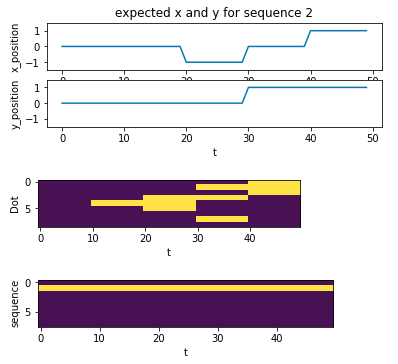
\includegraphics[scale=0.7]{fig13.png}
	\caption{یک نمونه ورودی و خروجی مطلوب شبکه (متناظر با دنباله‌ی شماره ۲)}
	\label{fig13}
\end{figure}

\subsection{پیاده‌سازی تسک}
با اعمال ورودی‌های متناظر به شبکه، آن را آموزش می‌دهیم. دقت کنید که دو ماتریس $9\times n$ و $8\times n$ برای ورود به شبکه به هم متصل شده‌اند و یک ماتریس $17\times n$ را تشکیل داده‌اند. برای بررسی عملکرد شبکه روی داده‌های تست، دو روش مورد استفاده قرار گرفته شده است. 
\begin{itemize}
	\item روش اول:\\
	تمام ۱۷ ورودی موجود در فرایند آموزش به شبکه داده می‌شود. انتظار داریم که خروجی در این حالت، از کیفیت بالایی برخوردار باشد. این وضعیت را به ازای دو حالت بررسی می‌کنیم؛ یک بار تعداد نورون‌های شبکه را کم در نظر می‌گیریم و بار دیگر تعداد نورون‌ها را بیشتر قرار می‌دهیم. در هر حالت، یک نمونه از نتایج شبکه بر روی دیتای آموزش و دیتای تست در این گزارش آورده شده است. شکل‌های \ref{fig14} تا \ref{fig17} نشان‌دهنده‌ی این خروجی‌ها هستند.
	
	\begin{figure}[h!]
		\centering
		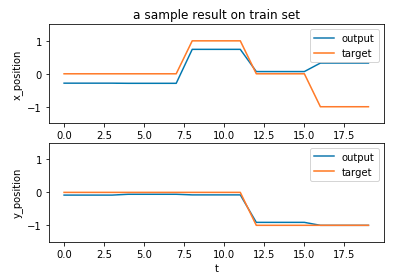
\includegraphics[scale=0.7]{fig14.png}
		\caption{یک نمونه از خروجی‌های شبکه با تعداد نورون‌های کم بر روی داده‌ی آموزش}
		\label{fig14}
	\end{figure}
	
		\begin{figure}[h!]
		\centering
		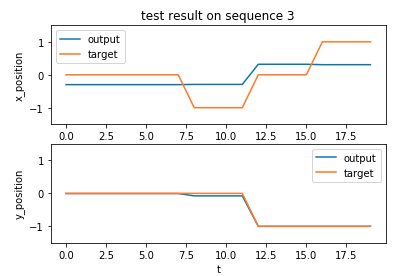
\includegraphics[scale=0.7]{fig15.png}
		\caption{یک نمونه از خروجی‌های شبکه با تعداد نورون‌های کم بر روی داده‌ی تست}
		\label{fig15}
	\end{figure}
	
		\begin{figure}[h!]
		\centering
		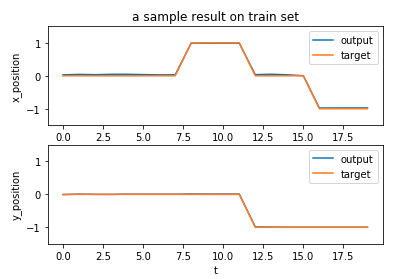
\includegraphics[scale=0.7]{fig16.png}
		\caption{یک نمونه از خروجی‌های شبکه با تعداد نورون‌های زیاد بر روی داده‌ی آموزش}
		\label{fig16}
	\end{figure}
	
		\begin{figure}[h!]
		\centering
		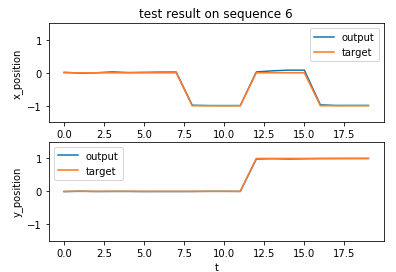
\includegraphics[scale=0.7]{fig17.png}
		\caption{یک نمونه از خروجی‌های شبکه با تعداد نورون‌های زیاد بر روی داده‌ی تست}
		\label{fig17}
	\end{figure}
مشاهده می‌شود که وقتی تعداد نورون‌ها زیاد می‌شود، نتایج قابل قبولی روی هر دو داده‌ی آموزش و تست به دست می‌آید.


	\item روش دوم:\\
در این حالت تنها ورودی‌های مربوط به مکان (ورودی‌های ۱ تا ۹) به شبکه داده می‌شود و دیگر نوع دنباله مشخص نمی‌شود. دو نمونه ورودی از نتایج حاصل بر روی دیتای آموزش و تست (برای شبکه با تعداد نورون‌های کافی) در شکل‌های \ref{fig18} و \ref{fig19} قابل مشاهده است.
\begin{figure}[h!]
	\centering
	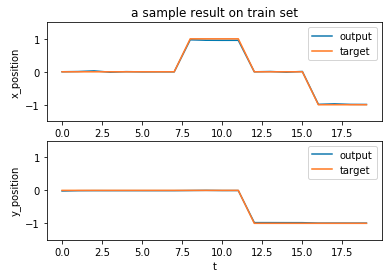
\includegraphics[scale=0.7]{fig18.png}
	\caption{یک نمونه از خروجی‌های شبکه بر روی داده‌ی آموزش بدون اعمال ورودی مربوط به نوع دنباله}
	\label{fig18}
\end{figure}

\begin{figure}[h!]
	\centering
	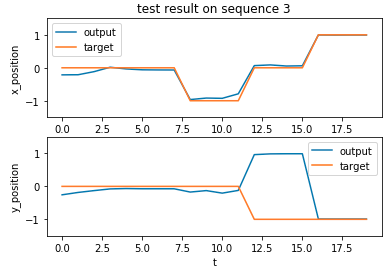
\includegraphics[scale=0.7]{fig19.png}
	\caption{یک نمونه از خروجی‌های شبکه بر روی داده‌ی تست بدون اعمال ورودی مربوط به نوع دنباله}
	\label{fig19}
\end{figure}

	مشاهده می‌شود که در این حالت، مجدداً نتایج مربوط به دیتای آموزش خوب است (که در واقع بخش مربوط به دیتای آموزش با روش اول تفاوتی ندارد)، اما بخش مربوط به دیتای تست به خوبی قبل نیست و شبکه بعضاً در تشخیص بعضی حرکات دچار اشتباه می‌شود و تصمیم نادرست می‌گیرد.
\end{itemize}




\end{document}

